\documentclass[12pt]{article}

% Linguagem
%\usepackage[portuguese]{babel}

% Clickable Table of contents
\usepackage{hyperref}
\hypersetup{
	hidelinks=true,
	colorlinks=true,
	linkcolor=DarkGreen!20!LightGreen!25!
}

% Table of contents
%\usepackage{tocloft}
%\setlength{\cftsubsecnumwidth}{3em} % Fix subsection width
% Fix space between subsection items on toc
%\renewcommand\cftsubsecafterpnum{\vskip5pt}

% Multicols
%\usepackage{multicol}

% Customize Chapter
\usepackage{titlesec}

\titleformat{\chapter}[hang]{\Huge\bfseries\color{DarkGreen!75!}}{\thechapter\hspace{20pt}{$|$}\hspace{20pt}}{0pt}{\Huge\bfseries}

% Appendix
%\usepackage{appendix}

% Maths
%\usepackage{amssymb} 		
%\usepackage{amsmath} 
%\usepackage[utf8]{inputenc} %useful to type directly diacritic characters

%\newcommand{\bm}[1]{{\boldmath{\large{\begin{align*} #1 \end{align*}}}}}

% Vectors
%\usepackage{esvect} 	% Vector over-arrow
%\usepackage{tikz}		% Vector diagrams
%\usetikzlibrary{calc}  % Vector calculations
%\usepackage{varwidth}  % List inside TikzPicture

%\renewcommand{\vec}{\vv} % Vecto over-arrow

% Chem
%\usepackage{chemformula} 	% formulas quimicas
%\usepackage{chemfig} 		% Estruturas quimicas

% Colors
\usepackage{xcolor}

\definecolor{DarkBlue}	{HTML}{252A36}
\definecolor{LightGreen}{HTML}{7CCC6C}
\definecolor{DarkGreen}	{HTML}{008675}

\pagecolor{DarkBlue!110!}
\color{DarkGreen!20!}

\usepackage{graphicx}

%\definecolor{Red}  {hsb}{0  ,.6,1}
%\definecolor{Blue} {hsb}{0.6,.6,1}
%\definecolor{Green}{hsb}{0.3,.6,1}

% Counters
%\counterwithin*{section}{part} % Reset section on part

% Resolução de listas
\renewcommand\thesection{Pergunta \arabic{section} }
\renewcommand\thesubsection{\arabic{section}-\alph{subsection}) }

\begin{document}

\setcounter{section}{22}
\section{}

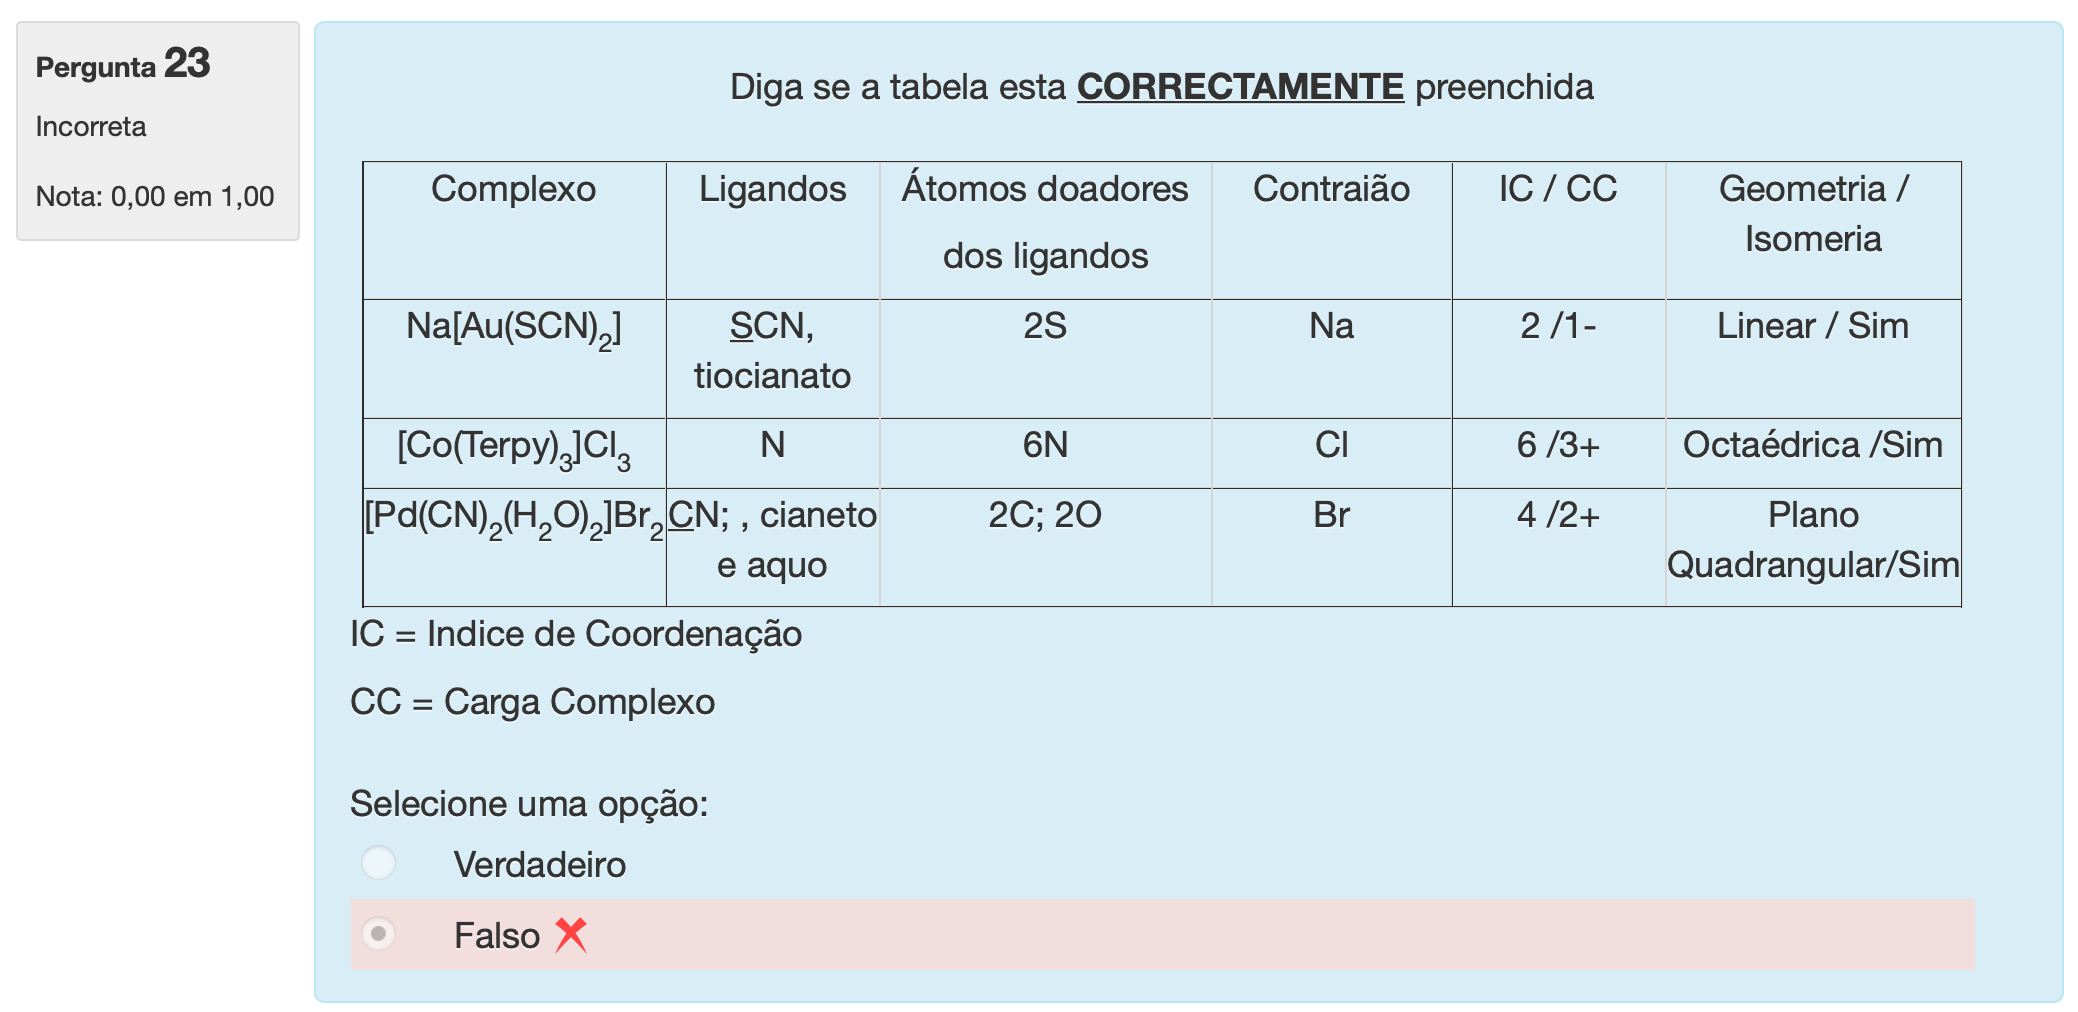
\includegraphics[width=\textwidth]{img2}

Nessa tabela o escrito como ligando é o azoto quando na realidade é a Terpiridina implicando que a tabela esteja incorretamente preenchida.

\setcounter{section}{28}
\section{}

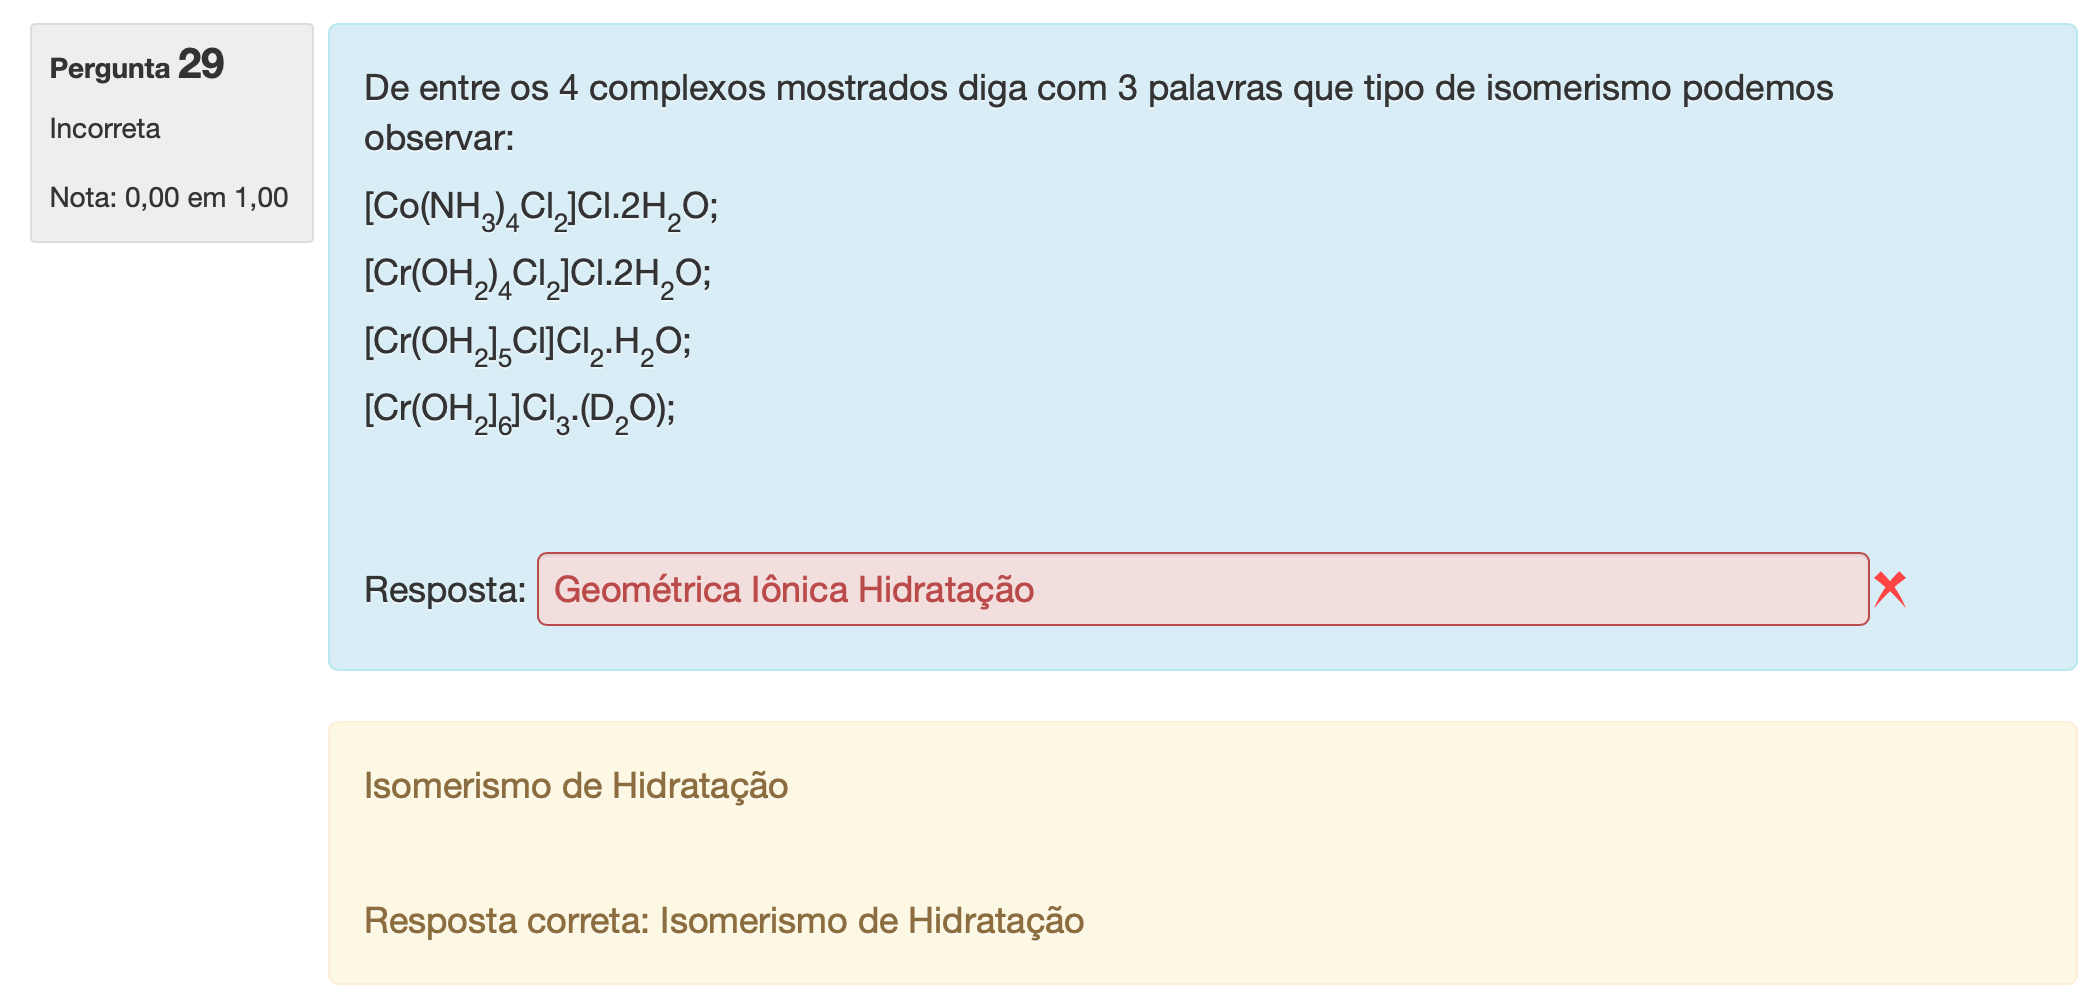
\includegraphics[width=\textwidth]{img1}

Aqui a pergunta está mal formulada, entende-se que se deve citar os tipos de isomerismo presente, não o comum entre todos os compostos.

\setcounter{section}{8}

\section{}
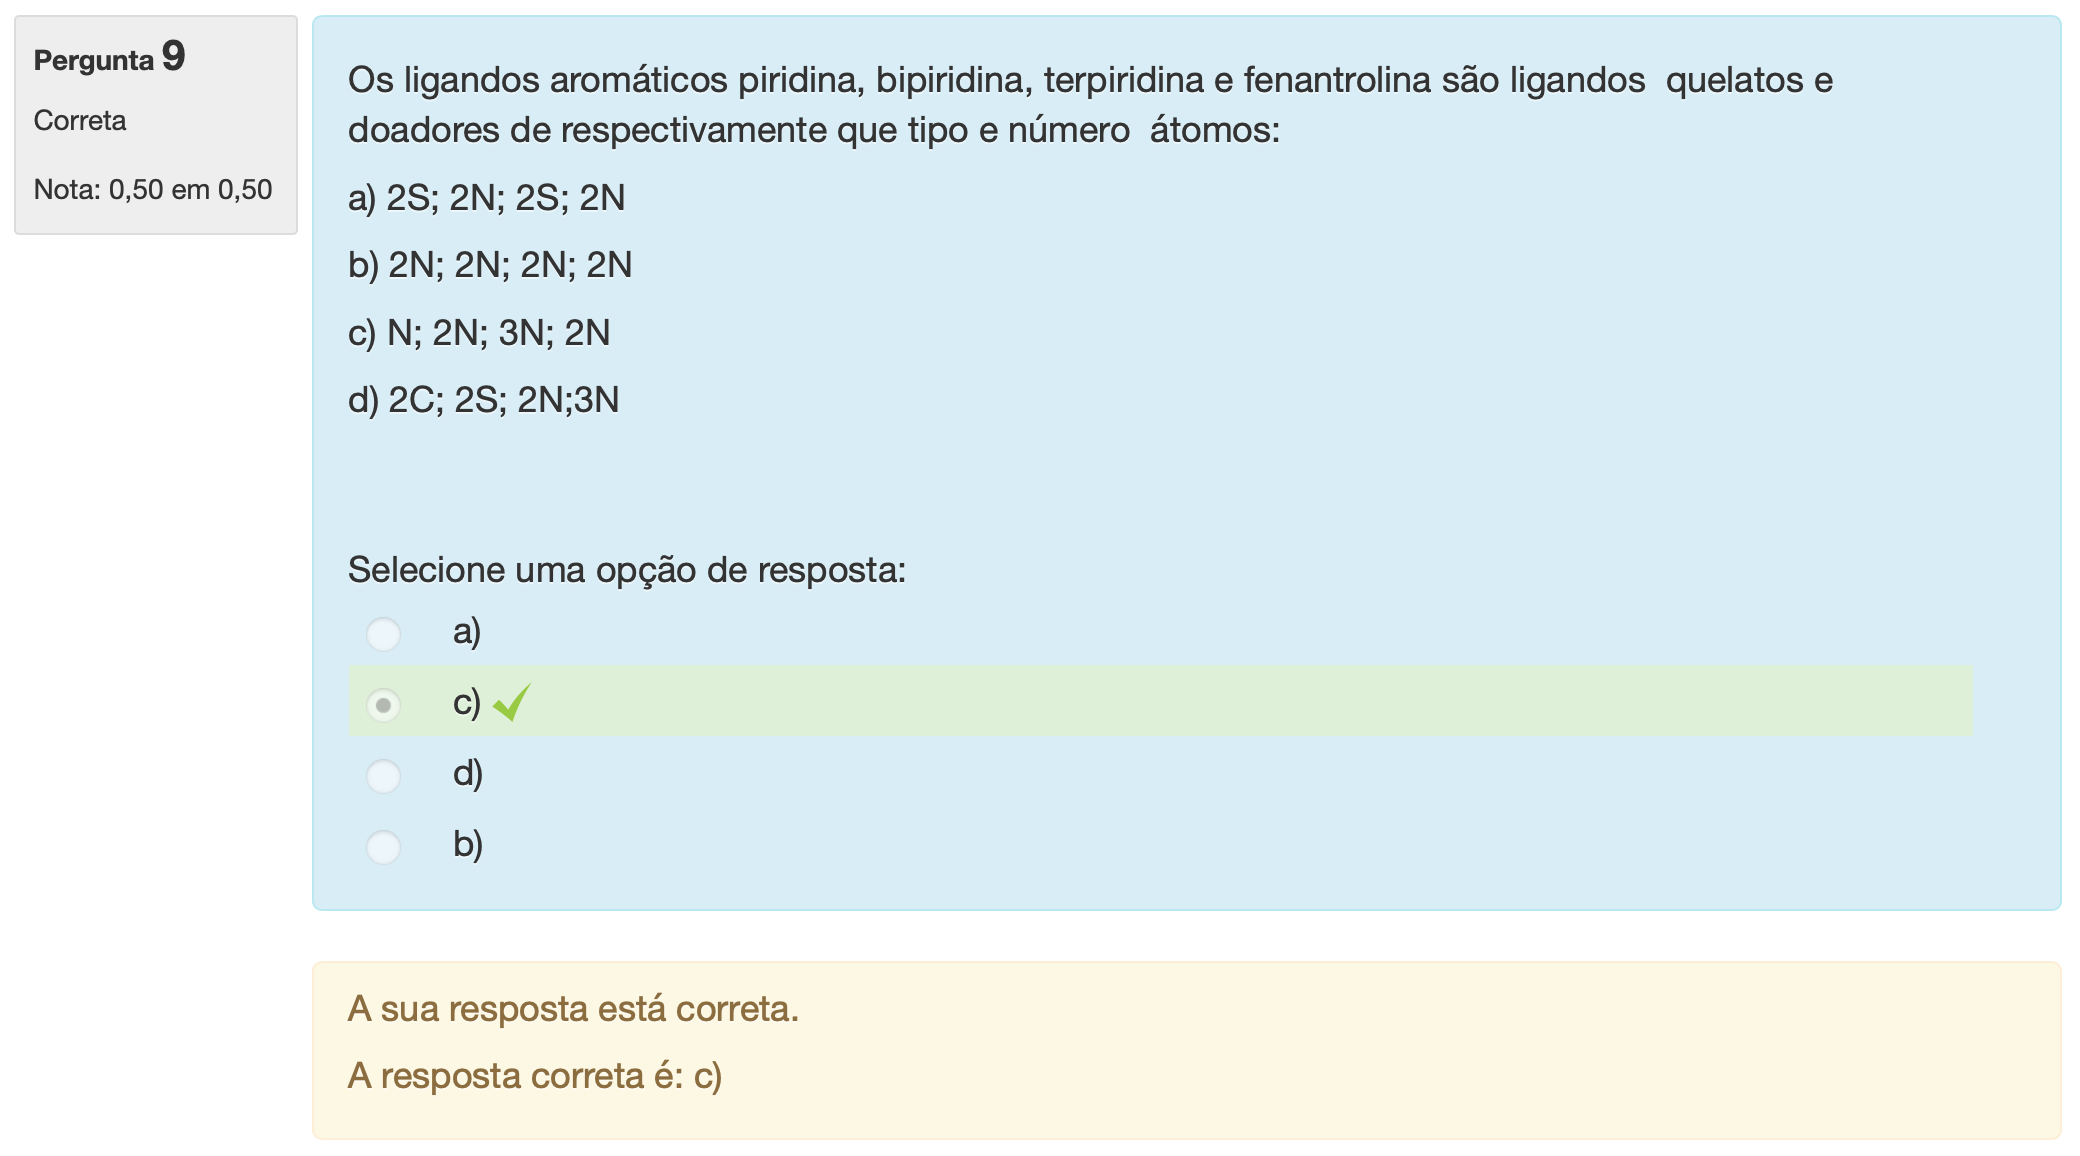
\includegraphics[width=\textwidth]{img3}

Esta questão está correta, so gostaria de apontar um pequeno erro no enunciado, onde nele de diz que a piridina é um ligando quelato, porem a piridina é monodentado e por isso não forma anel de quelação

\end{document}








